\section{Gefüllte Mangoldblätter mit Mango:ldchutney in Spinatschüsseln}
\begin{tikzpicture}[remember picture,overlay]
    \node[anchor=east,yshift=-4.5cm,inner sep=0pt] at (current page text area.east|-0,3cm) {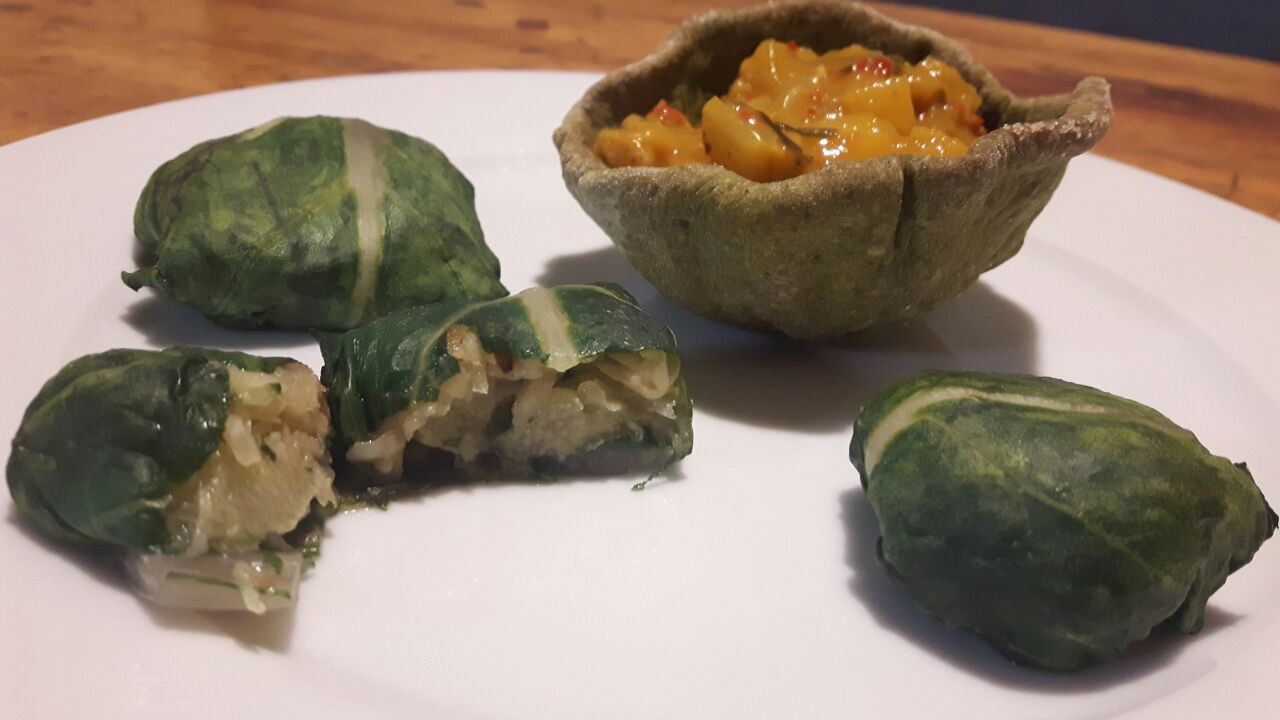
\includegraphics[height=4cm]{res/mango*ld.jpeg}};
\end{tikzpicture}
\subsection*{Spinaschüsseln}\label{subsec:spinach-bowls}
\begin{longtable}{rlL{17.1cm}}
    50g     &   Spinat          &   mit etwas   \\
            &   Wasser          &   pürieren und    \\
    1 EL    &   Sauerteigansatz &   dazugeben.  \\
            &   Weizenmehl      &   einkneten, bis der Teig pizzaartige Konsistenz hat.
                                    Über Nacht gehen lassen   \\
    1 TL    &   Salz            &   unterkneten.    \\
\end{longtable}
Ofen auf \cel{200} vorheizen.
Einen Apfel (oder etwas anderes Rundes von etwa gleicher Größe) zur Hälfte in Alufolie einwickeln, um kleine (gleichmäßige) Schüsseln daraus zu formen.
Den Teig zu kleinen Kugeln formen, plattdrücken und mit \textbf{ganzen Spinatblättern} belegen.
Fertig ausrollen und auf die mit Aluschüsseln legen und so für \mins{10} backen.
Die Aluschüsseln herausnehmen und die Teigschüsseln mit der Öffnung nach oben für weitere \mins{5--10} backen.

\subsection*{Mango*ldchutney}\label{subsec:chutney}
\begin{longtable}{rlL{16.2cm}}
    1               &   Mangold         &   putzen und die Blätter vom Stiel trennen.
                                            Die Stiele klein würfeln (ca. 2cm$^2$) zusammen mit \\
    1               &   Zwiebel         &   und \\
    1cm             &   Ingwer          &   für \mins{ca. 10} in  \\
    1--2 EL         &   Butter\footnote{gerne auch vegan z.B. \href{https://www.bio123.de/produkt/naturli/naturli-organic-vegan-block-200g}{Naturli vegan block}
									        oder \href{https://www.alsan.de/alsan-bio/}{Alsan}}
                                        &   anschwitzen.    \\
    1               &   Chili           &   in \\
    1 TL            &   Tomatenmark\footnote{Das Tomatenmark hilft dabei, die Chili besser schneiden zu können, ohne dass die Kerne wegspringen.}
                                        &   zu einem feinen Muß schneiden und hinzugeben.   \\
    $\frac{1}{2}$   &   Mango           &   Würfeln und dazugeben.  \\
    1 TL            &   Zitronensaft    &   und \\
    2--3 EL         &   Apfel-Mango-Saft\footnote{oder ein anderer passender Saft}
                                        &   hinzugeben und weitere \mins{10} köcheln lassen.
                                            Salzen und Pfeffern.    \\
\end{longtable}

\subsection*{gefüllte Mangoldblätter}\label{subsec:filled_chard}
\begin{longtable}{rlL{14.45cm}}
    Die                         &   Mangoldblätter      &   \mins{1} blanchieren.   \\
    200g ($\frac{1}{2}$ Knolle) &   Sellerie            &   schälen und reiben.
                                                            Dann zusammen mit   \\
    1                           &   Zwiebel             &   dünsten bis der Sellerie weich ist. \\
    1--2 Stangen                &   Rhabarber           &   schälen und in 1--2cm lange Stücke schneiden.
                                                            \mins{1--2} blanchieren. \\
    je 1                        &   Mangoldblatt        &   mit Selleriemasse ,,bestreichen'',  \\
    je $\frac{1}{2}$ TL         &   Dill                &   darauf verteilen, salzen und pfeffern,   \\
    je 1--2                     &   Rhabarberstückchen  &   darauf legen und mit    \\
    je 1 Prise                  &   Zimt                &   bestreuen.
                                                            Zufalten, sodass kleine Päckchen entstehen und für \mins{ca. 5} backen.  \\
\end{longtable}
Etwas \nameref{subsec:chutney} in die \nameref{subsec:spinach-bowls} geben und zusammen mit den \hyperref[subsec:filled_chard]{gefüllten Mangoldblättern} auf den Teller legen.